% 注释要用%开头,只提供整行注释

\documentclass[UTF8]{article} % 这句限制了整个文档的类型
% 类型就是包括标题啊章节啊等等在内的一套设定
% 比如你想写一个类似论文的东西,就用article就好了
% 前面的UTF8是编码方式
% 注意 反斜杠\后面的是函数,函数值中暂时可以认为调整参数写在[中括号里],内容在{大括号里}

\usepackage[zihao=-4]{ctex} % ctex可以写中文,中括号里那句的意思是正文小四号
\usepackage[a4paper]{geometry} % 调整纸张大小和页边距的包,这里中括号中规定了纸张大小
\usepackage{graphicx} % 用它在报告里加图
\usepackage{float}
\usepackage{indentfirst} % 用于首行缩进
\usepackage{listings}	% 代码插入
\usepackage{pythonhighlight} % python
\usepackage{xcolor}	% 颜色
\usepackage{url}	% url

\geometry{left=2.0cm,right=2.0cm,top=2.0cm,bottom=2.0cm} % 页边距设置
\setlength{\parindent}{2em} 	% 首行缩进2个中文字符

\definecolor{codegreen}{rgb}{0,0.6,0}
\definecolor{codegray}{rgb}{0.5,0.5,0.5}
\definecolor{codepurple}{rgb}{0.58,0,0.82}
\definecolor{backcolour}{rgb}{0.95,0.95,0.92}

\lstdefinestyle{python-editor}{
	language=python,
	backgroundcolor=\color{backcolour},   
	commentstyle=\color{codegreen},
	keywordstyle=\color{magenta},
	numberstyle=\tiny\color{codegray},
	stringstyle=\color{codepurple},
	basicstyle=\ttfamily\footnotesize,
	breakatwhitespace=false,         
	breaklines=true,                 
	captionpos=b,                    
	keepspaces=true,                 
	numbers=left,                    
	numbersep=5pt,                  
	showspaces=false,                
	showstringspaces=false,
	showtabs=false,                  
	tabsize=2
}



% 设置中英文摘要
\newcommand{\enabstractname}{Abstract}
\newcommand{\cnabstractname}{摘要}
\newenvironment{enabstract}{%
	\par\small
	\noindent\mbox{}\hfill{\bfseries \enabstractname}\hfill\mbox{}\par
	\vskip 2.5ex}{\par\vskip 2.5ex}
\newenvironment{cnabstract}{%
	\par\small
	\noindent\mbox{}\hfill{\bfseries \cnabstractname}\hfill\mbox{}\par
	\vskip 2.5ex}{\par\vskip 2.5ex}


% tile author date
%\title{电动汽车BMS设计与数字孪生的研究}
%\author{周密}
%\date{\today}

\begin{document}
	%% 封面设计
	% logo 中南大学
	\vspace*{1cm}
	\begin{figure}[htbp]
		\centering
		\graphicspath{{./images/}}
		
\includegraphics[width=0.7\linewidth]{logo}
	\end{figure}
	\vspace*{0.5cm}
	
	% 标题居中显示
	\begin{center}
		\Huge{\textbf{无线传感器网络技术课程实验报告}}
	\end{center}
	
	\vspace*{3.5cm}
	% 信息表格
	\begin{table}[h]
		\centering
		\begin{Large}
			\begin{tabular}{p{3cm} p{6cm}}
				姓\qquad 名:&  周密 \\
				\hline
				学\qquad 院:&  计算机学院\\
				\hline
				学\qquad 号:&  8210182308 \\
				\hline
				邮\qquad 箱: & zhoumicsu@csu.edu.cn\\
				\hline
				指导老师:& 张金焕\\
				\hline
				日\qquad 期:&  2021年12月2日早 \\
				\hline
			\end{tabular}
		\end{Large}
	\end{table}
	\thispagestyle{empty}       %本页不显示页码
	
	\clearpage
	%% title
	%\maketitle
	
	%% 摘要
	\begin{cnabstract}
		无线传感器网络作为物联网的一部分,占据着极为重要的作用,本课程实验基于Python编程语言,并且着手于网络的拓扑结构和网络分簇协议部分,其中实验一使用均匀分布,建立了一个圆形拓扑网络结构,并且确定了网络的Sink节点,实验二实现了LEACH分簇协议,基于实验一建立的圆形拓扑网络结构,基于欧几里德距离完成了网络分簇,并且基于能量消耗模型完成了对LEACH分簇协议低能耗效果的仿真。
		\par\textbf{关键词: } 无线传感器网络; 网络拓扑结构; Python; LEACH协议; 网络能量;%“\par在段首,表示另起一行,“\textbf{}”,花括号内的内容加粗显示
	\end{cnabstract}
	\begin{enabstract}
		As a part of the Internet of things, wireless sensor networks play a very important role. The experiment of this course is based on python programming language and focuses on the network topology and network clustering protocol. Experiment 1 uses uniform distribution to establish a circular topology network structure and determine the sink nodes of the network. Experiment 2 implements leach clustering protocol, Based on the circular topology network structure established in Experiment 1, the network clustering is completed based on Euclidean distance, and the low energy consumption effect of leach clustering protocol is simulated based on energy consumption model.
		\par\textbf{Keywords:}Wireless sensor network; Network topology; Python;  Leach agreement; Network energy;
	\end{enabstract}
	\thispagestyle{empty}       %本页不显示页码
	\clearpage
	
	%% 目录
	\tableofcontents
	\thispagestyle{empty}       %本页不显示页码
	\clearpage
	
	\setcounter{page}{1}        %从下面开始编页,页脚格式为导言部分设置的格式
	%% 正文内容
	
	\section{实验一:生成网络拓扑结构}
	\subsection{实验目的与要求}
	
	随机生成一圆形无线传感器网络,其中汇聚节点Sink位于圆心位置,半径为R,节点个数为N,节点发射和感知半径为r。
	要求:
	
	1. 网络中节点位置参数保存,可多次使用;
	
	2. 根据参数,绘出网络拓扑结构图;
	
	\subsection{实验内容、结果与分析}
	1. 生成圆形网络拓扑结构
	
	 随机生成圆形无线传感器网络,其中汇聚节点Sink位于圆心位置,半径$R$设为10,节点个数$N$为100,节点发射和感知半径为 $r$为10。实验结果如图\ref{fig:figure1}所示。
	 
	 通过python的随机数生成函数,首先生成$-1~+1$内均匀分布的两个随机数,分别用作某特定节点的横纵坐标,然后放大到$-R~+R$范围内,最后通过筛选除横纵坐标距离离Sink/坐标原点距离不大于R的坐标点作为节点的坐标,再重复成功生成$N-1$个节点,即完成圆形网络拓扑结构的生成。
	 
	 通过调用python中的散点图绘制函数scatter、以及折线图绘制函数plot完成整个网络的绘制和显示。
	
	\begin{figure}[H]
		\centering
		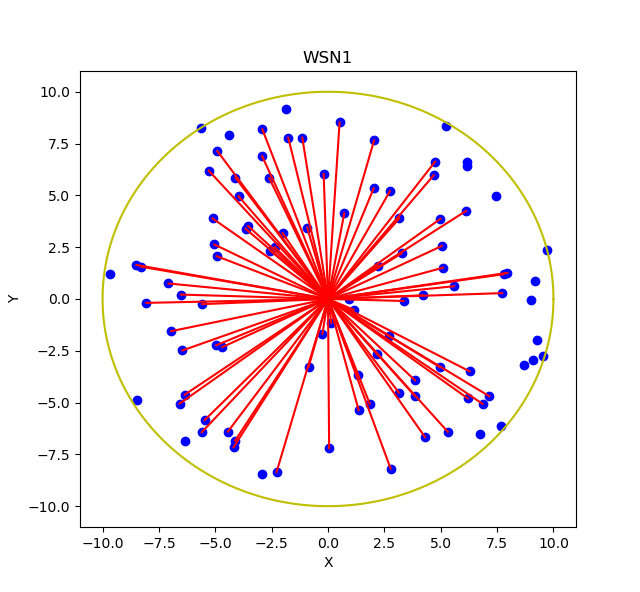
\includegraphics[width=0.7\linewidth]{Figure_1}
		\caption{未分簇的圆形拓扑无线传感器网络,Sink节点位于坐标原点,网络半径为10,通信半径为8.7}
		\label{fig:figure1}
	\end{figure}

	2. 保存生成的网络拓扑结构
	
	本文实现了网络拓扑结构节点位置的存储,存储的文件名为"top.txt",其中一行为一个坐标点,使用","分隔,而不同节点坐标之间使用换行符分隔,实验结果如图\ref{fig:screenshot004}所示。
	
	使用python的常用数据处理库numpy即可完成二维list的存储功能。
	
	\begin{figure}[H]
		\centering
		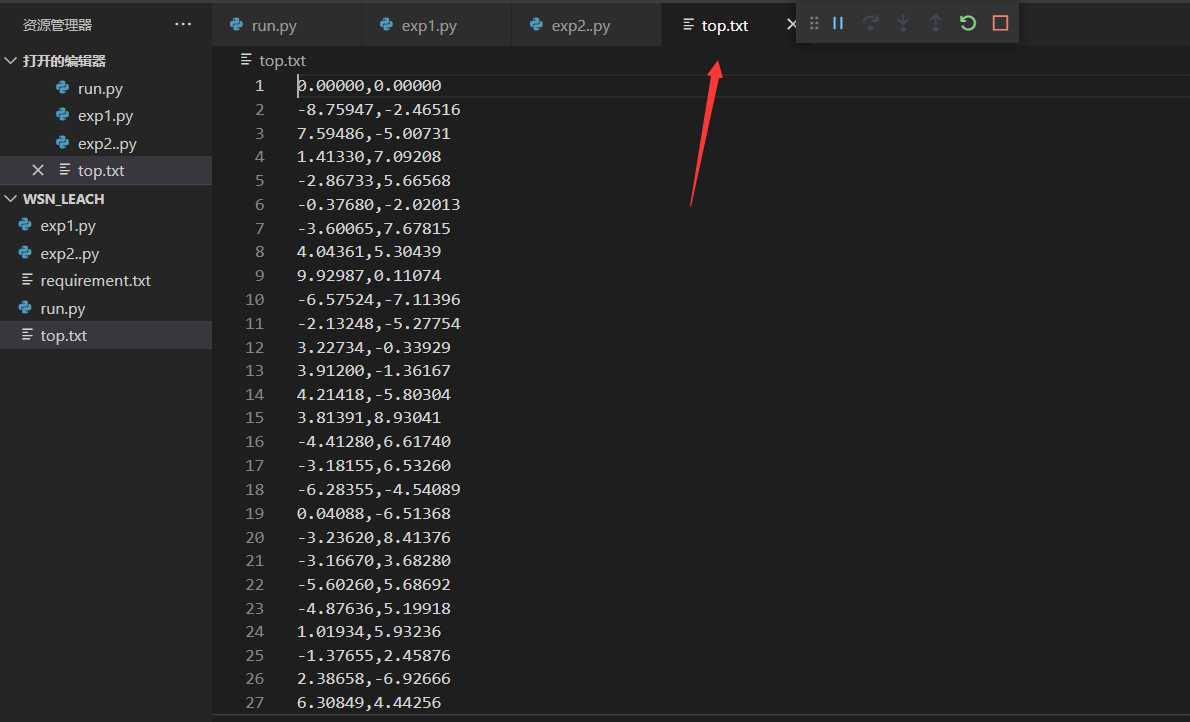
\includegraphics[width=0.7\linewidth]{screenshot004}
		\caption{网络拓扑结构保存为top.txt文件}
		\label{fig:screenshot004}
	\end{figure}

	\begin{figure}[H]
		\centering
		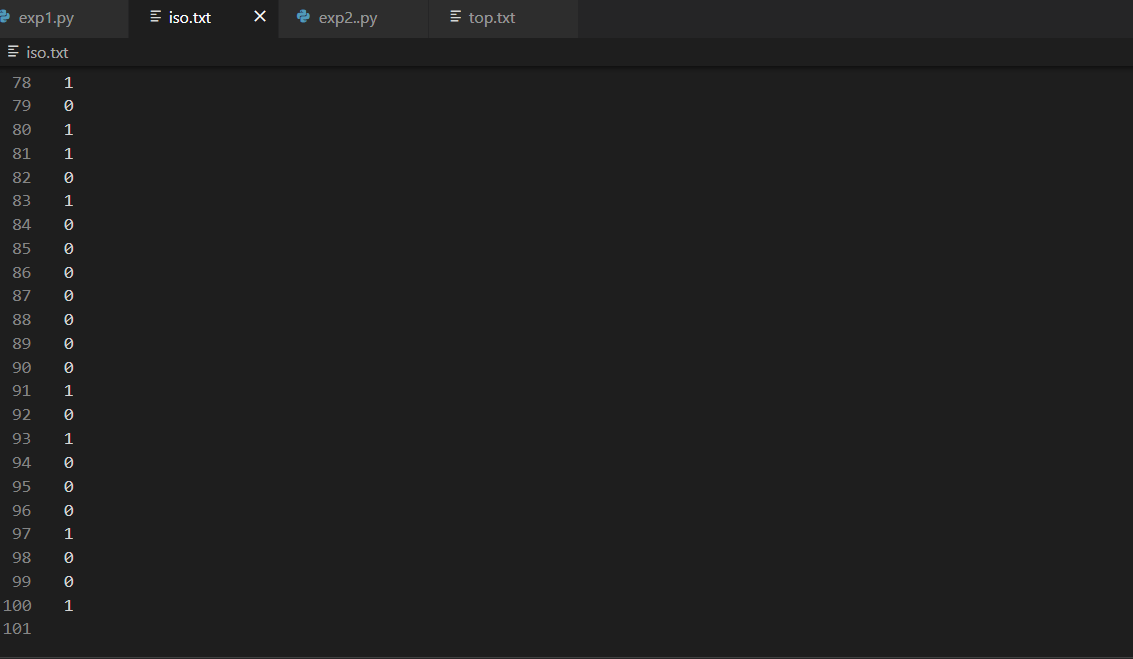
\includegraphics[width=0.7\linewidth]{screenshot005}
		\caption{网络中节点是否为孤立节点的标志保存为iso.txt}
		\label{fig:screenshot005}
	\end{figure}
	

	\subsection{实验代码}
	特此说明:本文实验一、实验二代码参考了csdn博客,但是做了必要的修改:\url{https://blog.csdn.net/wsh596823919/article/details/79981408}
	\begin{lstlisting}[style=python-editor]
		import numpy as np
		import matplotlib.pyplot as plt
		import turtle
		
		def run():
		"""
		1、node_factory(N, R, r): 生成N个节点的列表, 拓扑半径为R,通信半径r
		2、show_plt(top, iso, R): 迭代每次聚类结果,显示连线图
		:return:
		"""
			# 节点数目和圆形网络半径
			N = 100
			R = 10
			r = 8.7
			# 获取初始节点列表
			top, iso = node_factory(N, R, r)
			
			# 显示拓扑结构
			show_plt(top, iso, R)
		
			# 保存拓扑结构为txt文件
			save_top(top, iso)
		
		def dist(v_A, v_B):
		"""
		判断两个节点之间的欧几里得距离
		:param v_A: A 二维向量
		:param v_B: B 二维向量
		:return: 一维距离
		"""
			return np.sqrt(np.power((v_A[0] - v_B[0]), 2) + np.power((v_A[1] - v_B[1]), 2))
		
		def node_factory(N, R, r):
		"""
		生成N个节点的集合
		:param N: 节点的数目
		:param R: 圆形拓扑半径
		:param r: 节点通信半径
		:param nodes: 节点的集合
		:param iso: 标志:是否为孤立节点
		:return: 节点集合nodes=[[x,y],[x,y]...] + 标志iso
		"""
			nodes = []
			iso = []
			
			sinknode = [0, 0]
			nodes.append(sinknode)
			iso.append(0)
			
			i = 0
			while i < N-1:
				# 在1*1矩阵生成[x,y]坐标,并根据离sink节点的距离做判断是否为孤立节点
				node = [np.random.uniform(-1, 1)*R, np.random.uniform(-1, 1)*R]
				if dist(node, sinknode) < R and dist(node, sinknode) > r:
					nodes.append(node)
					iso.append(1)
					i = i + 1
				elif dist(node, sinknode) < R and dist(node, sinknode) < r:
					nodes.append(node)
					iso.append(0)
					i = i + 1
		
		
		return nodes, iso
		
		
		def show_plt(top, iso, R):
		"""
		显示分类图
		:param top: [[类1...],[类2...]....]-->[簇首,成员,成员...]
		:return:
		"""
			fig = plt.figure()
			ax1 = plt.gca()
			
			# 设置标题
			ax1.set_title('WSN1')
			# 设置X轴标签
			plt.xlabel('X')
			# 设置Y轴标签
			plt.ylabel('Y')
			
			for i in range(len(top)):
				plt.scatter(top[i][0], top[i][1], color='b')
				if i != 0 and iso[i] != 1:
					plt.plot([top[0][0], top[i][0]], [top[0][1], top[i][1]], color='r')
			
			a, b = (top[0][0], top[0][1])
			theta = np.arange(0, 2*np.pi, 0.01)
			x = a + R * np.cos(theta)
			y = b + R * np.sin(theta)
			plt.plot(x, y, 'y')
			plt.show()
		
		def save_top(top, iso):
		"""
		:param top: 网络拓扑结构
		:param iso: 是否为孤立节点标志
		"""
			np.savetxt('top.txt', top, fmt='%.5f', delimiter=',')
			np.savetxt('iso.txt', iso, fmt='%d', delimiter=',')
		
		if __name__ == '__main__':
			run()
	\end{lstlisting}
	
	\section{实验二:无线传感器网络LEACH协议}
	\subsection{实验目的与要求}
	根据实验1中的网络拓扑及其参数,实现LEACH分簇协议。
	
	要求:在一轮数据收集中
	
	1. 标绘出网络拓扑中的簇头节点;
	
	2. 标绘出每个簇头的簇成员。
	
	根据实验2中的分簇,统计LEACH协议允许的结果,假设数据包的大小为L,能量消耗模型为:
	\begin{figure}[H]
		\centering
		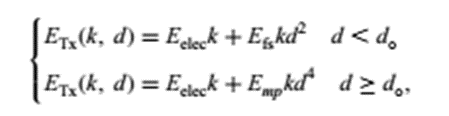
\includegraphics[width=0.5\linewidth]{screenshot001}
		\caption{网络能量消耗模型(发送方)}
		\label{fig:screenshot001}
	\end{figure}

	\begin{figure}[H]
		\centering
		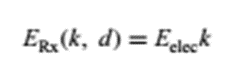
\includegraphics[width=0.3\linewidth]{screenshot002}
		\caption{网络能量消耗模型(接收方)}
		\label{fig:screenshot002}
	\end{figure}

	\begin{figure}[H]
		\centering
		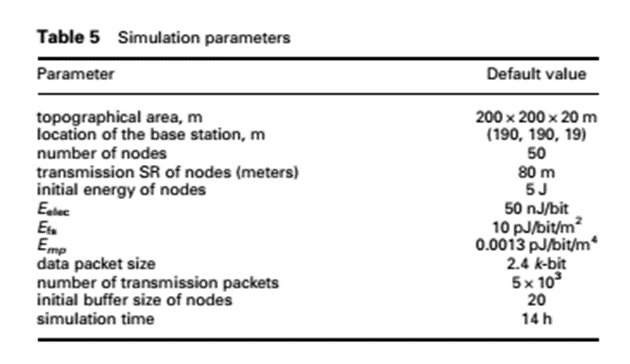
\includegraphics[width=0.7\linewidth]{screenshot003}
		\caption{网络模型参数参考}
		\label{fig:screenshot003}
	\end{figure}

	要求:在一轮数据收集中,每个节点都产生一个数据包,并汇聚到Sink节点
	
	1.	统计每个节点发送和 接收的数据包个数,并直观显示出来;
	
	2. 统计每个节点能量消耗,并给出三维能量消耗图。

	\subsection{实验内容、结果与分析}
	1. 绘制网络拓扑的簇头节点及其簇成员
	
	在完成整个网络拓扑结构的建模之后,通过LEACH算法可以对网络中的节点进行分簇。对于LEACH,这里有必要对它做一些必要的介绍:
	
	 LEACH来源于Wendi Rabiner Heinzelman, Anantha Chandrakasan, 和Hari Balakrishnan三人在2000年Proceedings of the 33rd Hawaii International Conference on System Sciences上的一篇文章Energy-Efficient Communication Protocol forWireless Microsensor Networks。
	 
	 LEACH协议全称是“低功耗自适应集簇分层型协议” (Low Energy Adaptive Clustering Hierarchy)。
	  
	 该算法基本思想是:以循环的方式随机选择蔟首节点,将整个网络的能量负载平均分配到每个传感器节点中,从而达到降低网络能源消耗、提高网络整体生存时间的目的。仿真表明,与一般的平面多跳路由协议和静态分层算法相比,LEACH协议可以将网络生命周期延长15\%。
	  
	 LEACH在运行过程中不断的循环执行蔟的重构过程,每个蔟重构过程可以用回合的概念来描述。每个回合可以分成两个阶段:蔟的建立阶段和传输数据的稳定阶段。为了节省资源开销,稳定阶段的持续时间要大于建立阶段的持续时间。蔟的建立过程可分成4个阶段:蔟首节点的选择、蔟首节点的广播、蔟首节点的建立和调度机制的生成。
	  
	 蔟首节点的选择依据网络中所需要的蔟首节点总数和迄今为止每个节点已成为蔟首节点的次数来决定。具体的选择办法是:每个传感器节点随机选择$0~1$之间的一个值。如果选定的值小于某一个阀值,那么这个节点成为蔟首节点。
	  
	 选定蔟首节点后,通过广播告知整个网络。网络中的其他节点根据接收信息的信号强度决定从属的蔟,并通知相应的蔟首节点,完成蔟的建立。最后,蔟首节点采用TDMA方式为蔟中每个节点分配向其传递数据的时间点。
	  
	 稳定阶段中,传感器节点将采集的数据传送到蔟首节点。蔟首节点对蔟中所有节点所采集的数据进行信息融合后再传送给汇聚节点,这是一种叫少通信业务量的合理工作模型。稳定阶段持续一段时间后,网络重新进入蔟的建立阶段,进行下一回合的蔟重构,不断循环,每个蔟采用不同的CDMA代码进行通信来减少其他蔟内节点的干扰。
	  
	 LEACH协议主要分为两个阶段:即簇建立阶段(setup phase)和稳定运行阶段(ready phase)。簇建立阶段和稳定运行阶段所持续的时间总和为一轮(round)。为减少协议开销,稳定运行阶段的持续时间要长于簇建立阶段。
	  
	 在簇建立阶段,传感器节点随机生成一个0,1之间的随机数,并且与阈值T(n)做比较,如果小于该阈值,则该节点就会当选为簇头。参考csdn博客\url{https://blog.csdn.net/wangh0802/article/details/78656775}
	 
	 在这里,通过概率选取簇头, 形成簇头组成的list,随后对剩余的每一个节点,都要对簇头list进行遍历,找到离该节点最近的簇头,记录下该距离,并将该节点归入到该簇头的簇下。实验结果如图\ref{fig:figure2}和图\ref{fig:figure4}所示。
	 
	 \begin{figure}[H]
	 	\centering
	 	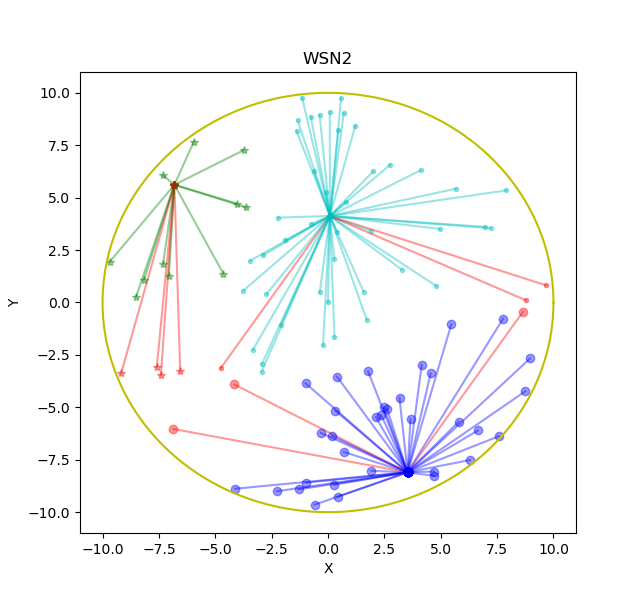
\includegraphics[width=0.65\linewidth]{Figure_2}
	 	\caption{使用LEACH分簇协议分簇后的网络结构(第一轮),连线表示节点隶属于哪一簇,红线连接表示超出通信半径r=8.7,此节点为该簇中的孤立节点}
	 	\label{fig:figure2}
	 \end{figure}
 
	 \begin{figure}[H]
	 	\centering
	 	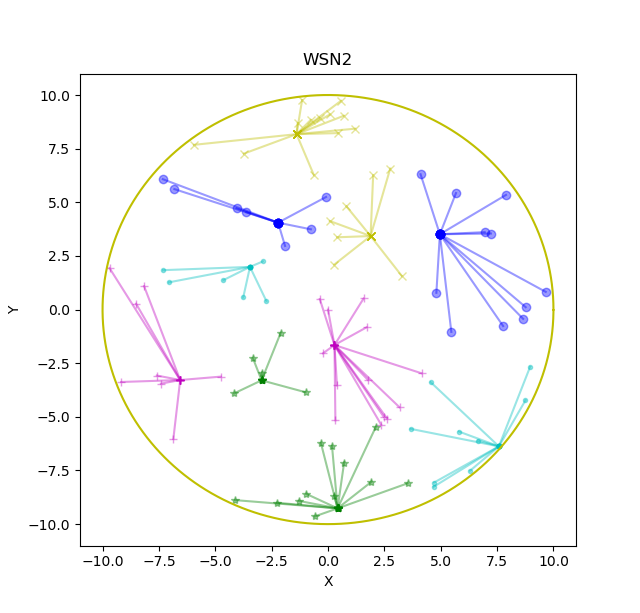
\includegraphics[width=0.65\linewidth]{Figure_4}
	 	\caption{使用LEACH分簇协议分簇后的网络结构(第二轮),连线表示节点隶属于哪一簇,红线连接表示超出通信半径r=8.7,此节点为该簇中的孤立节点}
	 	\label{fig:figure4}
	 \end{figure}
 
	 
	2. 数据包的发送以及能量仿真
	
	这里对实验内容做了一定的简化,只考虑了在完成分簇之后,各个簇中的节点向簇头发送数据的能量损失,而没有考虑其他的能量损失,但是这种简化是有一定道理的,在网络拓扑结构比较合理,在区域内分布比较均匀的情况下,实际上网络的绝大部分能量是由有效的数据包交换消耗的。因此我们忽略了一下能量消耗:在分簇时,各个节点在物理上实际上时彼此独立分隔的,然后要做到对于整个网络的自组织功能,实现网络按照特定算法分簇,是需要进行数据包交换的,即由能量的消耗。在每一簇内,当节点们把数据包传送给簇头时,我们只考虑单跳的情况,并且认为信道是时不变的理想的,并且我们认为所有的数据包的长度相同,数目也是稳定的。在完成从节点到簇中心的传送后,我们没有考虑到Sink节点的传送。所以综合以上几点,我们这里提出的仿真不是完整的仿真,而是多种近似、简化后的结果。
	
	在实验二的1中,我们可以获得每一个簇中的节点,并且可以得到簇到其中各个节点的距离,在获得该距离之后,我们即可通过上述提出的能量消耗模型进行仿真,值得注意的是:收发双方的能量消耗模型是不同的,并且发送方的能量消耗与距离有关,这一点是很直观的:当距离较远时,如果要保证一定的信噪比使得接收方能够成功恢复数据,那么就需要加大信号的发送功率。并且,这里我们对于每个节点不仅仅存储其坐标节点,我们同时保存了它的剩余能量值,以便此处进行网络能量的分析。
	
	对于每个簇中的孤立的节点,我们做这样的处理:能够发送数据按照发送数据包消耗能量模型进行处理,但是对于该节点所在的簇头节点来讲,并不会损耗能量。
	
	在出现第一个网络节点能量耗尽时,实验结果的三维能量分布图如图\ref{fig:figure3}所示。
	\begin{figure}[H]
		\centering
		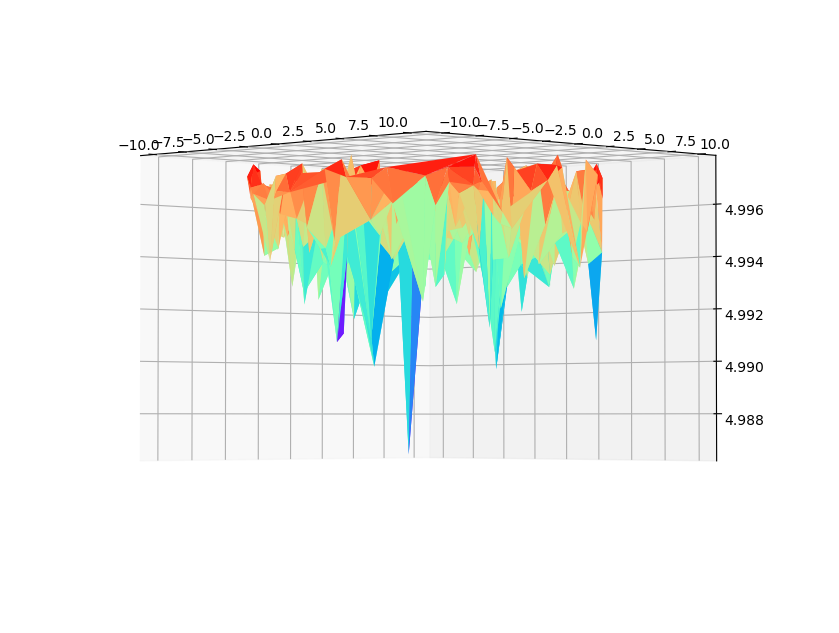
\includegraphics[width=0.7\linewidth]{Figure_3}
		\caption{在迭代循环1000次之后,各个节点的能量剩余三维图, 为了效果更好,这里使用500个节点}
		\label{fig:figure3}
	\end{figure}
	
		从之前的分析可以看出,LEACH算法存在的一定的缺点:在LEACH算法中,每一轮循环都要重新构造簇,而构造簇的能量开销比较大。其次,远离汇聚节点的簇头节点可能会由于长距离发送数据而过早耗尽自身能量,造成网络分割。另外,LEACH算法没有考虑簇头节点当前的能量状况,如果能量很低的节点当选为簇头节点,那么将会加速该节点的死亡,影响整个网络的生命周期。
	
	并且LEACH的使用存在一定的局限性:1. 由于LEACH假定所有节点能够与汇聚节点直接通信,并且每个节点都具备支持不同MAC协议的计算能力,因此该协议不适合在大规模的无线传感器网络中应用。2. 协议没有说明簇头节点的数目怎么分布才能及于整个网络。因此,很可能出现被选的簇头节点集中在网络某一区域的现象,这样就会使得一些节点的周围没有任何簇头节点。3. 由于LEACH假定在最初的簇头选择回合中,所有的节点都携带相同的能量,并且每个成为簇头的节点都消耗大致相同的能量。因此,协议不适合节点能量不均衡的网络。
	
	\subsection{实验代码}
	特此说明:本文实验一、实验二代码参考了csdn博客,但是做了必要的修改:\url{https://blog.csdn.net/wsh596823919/article/details/79981408}
	\begin{lstlisting}[style=python-editor]
		import numpy as np
		import matplotlib.pyplot as plt
		from mpl_toolkits.mplot3d import Axes3D
		
		
		def dist(v_A, v_B):
		"""
		判断两个节点之间的一维距离
		:param v_A: A 二维向量
		:param v_B: B 二维向量
		:return: 一维距离
		"""
			return np.sqrt(np.power((v_A[0] - v_B[0]), 2) + np.power((v_A[1] - v_B[1]), 2))
		
		
		def node_factory(N, R, r, energy=50):
		"""
		生成N个节点的拓扑网络
		:param N: 网络中节点个数
		:param R: 圆形拓扑半径
		:para r: 通信半径范围,超出此范围为某簇的孤立节点
		:param selected_flag: 标志:是否被选择为簇首-->初始化为0
		:param energy: 能量
		:return: 节点集合nodes=[[x,y,e],[x,y,e]...]
		"""
			nodes = []
			selected_flag = []
			iso = []
			
			# 中心sink节点
			sinknode = [0, 0, energy]
			nodes.append(sinknode)
			selected_flag.append(0)
			
			# 随机生成圆形拓扑网络
			i = 0
			while i < N-1:
				# 在1*1矩阵生成[x,y]坐标
				node = [np.random.uniform(-1, 1)*R, np.random.uniform(-1, 1)*R, energy]
				if dist(node, sinknode) < R and dist(node, sinknode) > r:
					nodes.append(node)
					selected_flag.append(0)
					iso.append(1)
					i = i + 1
				elif dist(node, sinknode) < R and dist(node, sinknode) < r:
					nodes.append(node)
					selected_flag.append(0)
					iso.append(0)
					i = i + 1
			
			
			return nodes, selected_flag, iso
		
		
		def sel_heads(r, nodes, flags):
		"""
		使用leach协议,选取簇头(注意这里还没有开始进入正式的分簇,这里只选了簇头)
		:param r: 轮数
		:param nodes: 节点列表
		:param flags: 选择标志
		:param P: 比例因子
		:return: 簇首列表heads,簇成员列表members
		"""
			# 阈值函数 Tn 使用leach计算
			P = 0.05 * (100 / len(nodes))
			Tn = P / (1 - P * (r % (1 / P)))
			heads = []  # 簇首列表
			members = []    # 簇成员列表
			n_head = 0  # 本轮簇首数
			rands = [np.random.random() for _ in range(len(nodes))] # 对每个节点生成对应的随机数,用于筛选簇头
			
			# 遍历随机数列表,选取簇首
			for i in range(len(nodes)):
				# 随机数低于阈值-->选为簇首
				if rands[i] <= Tn:
					flags[i] = 1
					heads.append(nodes[i])
					n_head += 1
				# 随机数高于阈值
				else:
					members.append(nodes[i])
			
			return heads, members
		
		
		def classify(nodes, flag, r, mode=1, k=20):
		"""
		对网络进行簇分类
		:param nodes: 节点列表
		:param flag: 节点标记
		:param mode: 0-->显示图片(死亡节点不显示)  1-->显示结束轮数
		:param k: 轮数
		:return: 簇分类结果列表 classes[[类1..],[类2...],......]  [类1...簇首...簇成员]
		"""
			# 能量损耗模型的参数
			b = 2400
			e_elec = 5*np.power(10., -9)
			e_fs = 10*np.power(10., -12)
			e_mp = 0.0013*np.power(10., -12)
			d_0 = 80
			
			# k轮的有效集合: 无死亡节点
			iter_classes = []
			# 是否已有节点能量为0
			e_is_empty = 0
			
			# 迭代r轮
			for r in range(k):
				# mode1: 若无死亡节点 继续迭代
				if e_is_empty == 0:
					# 获取簇首列表,簇成员列表
					heads, members = sel_heads(r,nodes,flag)
					
					# 建立簇类的列表
					if len(heads) == 0:
						break
					classes = [[] for _ in range(len(heads))]
					
					# 将簇首作为首节点添加到聚类列表中
					for i in range(len(heads)):
						classes[i].append(heads[i])
					
					# 簇分类:遍历节点node
					for member in members:
					
						# 选取距离最小的节点
						dist_min = 100000
						
						# 判断和每个簇首的距离
						for i in range(len(heads)):
						
							dist_heads = dist(member, heads[i])
						
							# 找到距离最小的簇头对应的heads下标i
							if dist_heads < dist_min:
							dist_min = dist_heads
							head_cla = i
						if dist_min==1:
							print("本轮没有簇首!")
							break
							# 添加到距离最小的簇首对应的聚类列表中
						
						classes[head_cla].append(member)
						
						# 正式的数据传输过程,使用能量消耗模型
						if int(member[2]) > 0 and int(heads[head_cla][2]) > 0:
							if dist_min < d_0:
								member[2] -= e_elec*b+e_fs*b*dist_min
							else:
								member[2] -= e_elec*b+e_mp*b*dist_min
							
							if dist([member[0], member[1]], [heads[head_cla][0], heads[head_cla][1]]) <= r:
								heads[head_cla][2] -= e_elec*b
							else:
								pass
						
						
							# heads[head_cla][2] -= e_elec*b
						else:
						e_is_empty = mode
						break
					iter_classes.append(classes)
				
				else:
					print("第", r, "轮能量耗尽")
					break
			
			return iter_classes
		
		
		def show_plt(classes, R, r):
		"""
		显示分类图
		:param classes: [[类1...],[类2...]....]-->[簇首,成员,成员...]
		:param R: 圆形拓扑半径
		:para r: 通信半径范围,超出此范围为某簇的孤立节点
		:return:
		"""
			fig = plt.figure()
			ax1 = plt.gca()
			
			# 设置标题
			ax1.set_title('WSN2')
			# 设置X轴标签
			plt.xlabel('X')
			# 设置Y轴标签
			plt.ylabel('Y')
			
			# 簇内的显示点图标及连线颜色,以得到较好的显示结果
			icon = ['o', '*', '.', 'x', '+', 's']
			color = ['b', 'g', 'c', 'y', 'm']
			
			x, y, e = [], [], []
			
			# 对不同的簇进行不同的显示,以得到较好的显示结果
			for i in range(len(classes)):
				centor = classes[i][0]
				x.append(centor[0])
				y.append(centor[1])
				e.append(centor[2])
				for point in classes[i]:
					if point[2] > 0 and dist(centor, point) < r:
						ax1.plot([centor[0], point[0]], [centor[1], point[1]], c=color[i % 5], marker=icon[i % 5], alpha=0.4)
					elif point[2] > 0 and dist(centor, point) > r:
						ax1.plot([centor[0], point[0]], [centor[1], point[1]], c='r', marker=icon[i % 5], alpha=0.4)
					else:
						pass
			
			
			a, b = (0., 0.)
			theta = np.arange(0, 2*np.pi, 0.01)
			x = a + R * np.cos(theta)
			y = b + R * np.sin(theta)
			plt.plot(x, y, 'y')
			
			# 显示
			plt.show()
		
		def show_eninfo(iter_classes):
			fig = plt.figure()
			ax1 = Axes3D(fig)
			lastclass = iter_classes[-1]
			
			x, y, e = [], [], []
			
			# 将所有节点的剩余能量统计起来,用于后续能量三维图的显示
			for i in range(len(lastclass)):
				centor = lastclass[i][0]
				x.append(centor[0])
				y.append(centor[1])
				e.append(centor[2])
				for point in lastclass[i]:
					if point[2] > 0:
						x.append(point[0])
						y.append(point[1])
						e.append(point[2])
					else:
						pass
			
			# 需要进行数据类型转换list->ndarray,才能进行三维图像的显示
			x = np.array(x)
			y = np.array(y)
			e = np.array(e)
			
			# 显示三维图像
			ax1.plot_trisurf(x, y, e, cmap='rainbow')
			plt.show()
		
		def run():
		"""
		"""
			# N = int(input("请输入节点个数:"))
			N = 500
			R = 10
			r = 8.7
			
			# 获取初始节点列表
			nodes, flag, iso = node_factory(N, R, r, energy=5)
			# 对节点列表进行簇分类,mode为模式 2种
			iter_classes = classify(nodes,flag, r, mode=1, k=200)
			# 迭代每次聚类结果,显示连线图
			for classes in iter_classes:
			     # 显示分类结果
			     show_plt(classes, R, r)
			
			show_eninfo(iter_classes)
		if __name__ == '__main__':
			run()
	\end{lstlisting}
	
	\section{实验总结与体会}
	\subsection{感悟}
	无线传感器网络的仿真工具有很多,之前老师推荐的时omnet++,omnet++作为专业的网络仿真开源工具,具有十分强大的功能。本文使用的是python语言直接作为开发语言,python作为一种解释性语言,十分容易上手,能够让开发者多关注实验业务方面,而不是纠结于语法。同时,python语言现在越来越流行,基于以上考虑,本文使用python作为开发语言。
	
	无线传感器网络的仿真中,我总结主要有几个重点内容:网络拓扑结构的建立,网络分簇协议的实现,网络转化路由协议的实现等,在本实验中,出于时间有限,所以主要内容是前两个相对容易的部分。
	
	1. 网络拓扑结构的建立
	
	需要用到python中的随机数生成的点:np.random.funciton(random()/uniform/......),用到欧几里德距离的计算,用到结构体、类等面向对象的概念,字典、列表等数据结构。
	
	2. 网络分簇协议的实现
	
	分簇协议类似于机器学习中属于无监督学习的聚类的方法,不过这里的分簇协议需要考虑数据包转发、能量效率等问题,而在聚类中只需要考虑距离。
	
	其中LEACH协议存在一定的缺点和局限性,在LEACH算法中,每一轮循环都要重新构造簇,而构造簇的能量开销比较大。其次,远离汇聚节点的簇头节点可能会由于长距离发送数据而过早耗尽自身能量,造成网络分割。另外,LEACH算法没有考虑簇头节点当前的能量状况,如果能量很低的节点当选为簇头节点,那么将会加速该节点的死亡,影响整个网络的生命周期。
	
	并且LEACH的使用存在一定的局限性:1. 由于LEACH假定所有节点能够与汇聚节点直接通信,并且每个节点都具备支持不同MAC协议的计算能力,因此该协议不适合在大规模的无线传感器网络中应用。2. 协议没有说明簇头节点的数目怎么分布才能及于整个网络。因此,很可能出现被选的簇头节点集中在网络某一区域的现象,这样就会使得一些节点的周围没有任何簇头节点。3. 由于LEACH假定在最初的簇头选择回合中,所有的节点都携带相同的能量,并且每个成为簇头的节点都消耗大致相同的能量。因此,协议不适合节点能量不均衡的网络。
	
	\subsection{收获}
	收获了python的编程技术的提升,收获了debug的能力,练习了latex写报告、论文的一些技巧,巩固了无线传感器网络课程的基础知识(如LEACH分簇协议等),了解和熟悉了无线传感器网络的仿真过程,以及使用编程语言实现它的方法。
	
	\end{document}